%!TEX root = ../master.tex

\section{Figures and Tables}
Here you will find examples of how to insert figures and tables.


\subsection{Experimental Design}

In the NO-FILTER condition, ten randomly chosen projects were shown to the participant on the overview page
(see Figure \ref{fig:overview}). There was a short description of each project on the list,
as well as a photo, the name, the amount of money already lent to the project
and one sentence describing the project. The participants could then click on
each project in any order to access the detailed project description page,
which described the project in a longer text of mostly two to three paragraphs (see Figure \ref{fig:procedure1}).
In addition, information was provided on the repayment schedule. The participants could navigate
between the overview page and the detailed description in any order and as long they wanted.
Finally, they had to choose one project by clicking on the “Choose” button in the detailed project description.\\
Condition STANDARD: Filter Followed by Joint Evaluation\\
In the STANDARD condition, participants could set filters for several criteria (see Figure \ref{fig:firststep}).
They were not forced to set filters, but all participants used them.
Subsequently, they were asked to rank the order of the filter criteria they selected according to their importance (see Figure \ref{fig:secondstep}).
Afterwards, they saw the same overview page and the detailed project description page as the participants in the NO-FILTER condition (see Figure \ref{fig:overview} (right) and Figure \ref{fig:procedure1}).
However, the ten projects they saw were not randomly chosen, but selected on the basis of their filters and importance sorting.\\
\begin{figure}[h]
    \centering
    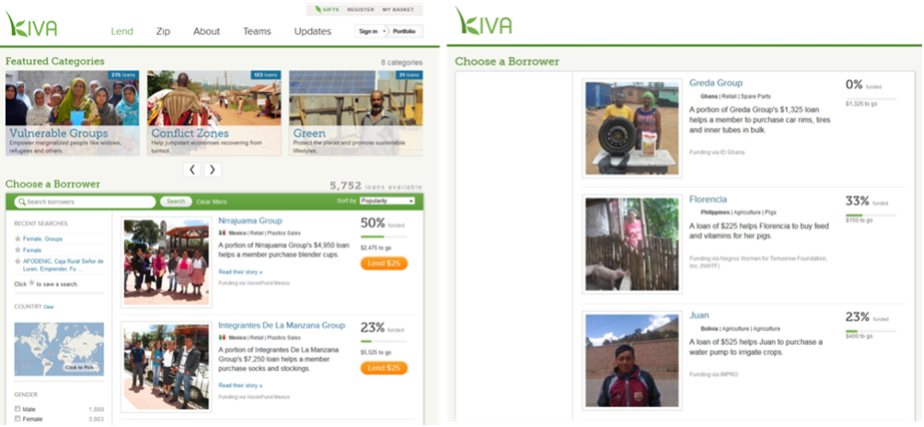
\includegraphics[width=0.8\textwidth]{graphics/Bild1}
    \caption{Overview page. Left: Original Screenshot from KIVA. Right: Screen that participants saw in the experiment (Overview Page).}
    \label{fig:overview}
\end{figure}

\begin{figure}[h]
    \centering
    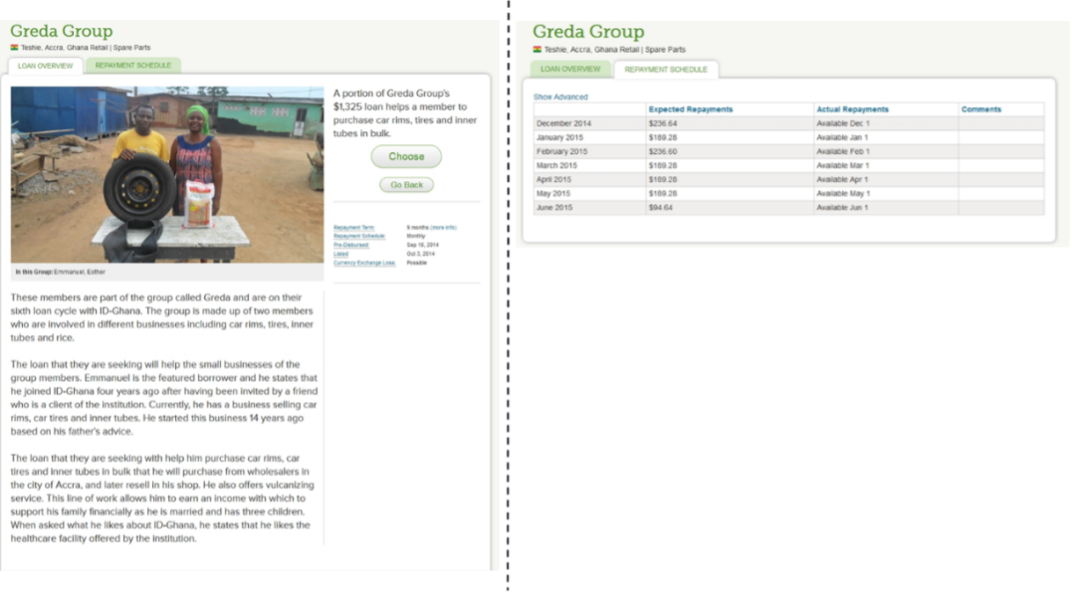
\includegraphics[width=0.8\textwidth]{graphics/Bild2}
    \caption{ Detailed Project Description Page with repayment schedule.}
    \label{fig:procedure1}
\end{figure}
As filter
criteria, the participants could set: country, gender, sector, groups or
individuals, and attributes (for example, green, start-up, youth, fair trade,
etc.). These are the same filters the KIVA offered on the standard screen at
the time of our experiment. If less than ten projects met the filter criteria,
the least importance criteria were relaxed. For example, if a participant had
set the two filters gender=females and sector=education and had indicated
sector as more important than gender, but only eight projects fulfilled both
criteria, we selected these eight projects and then selected another two
projects randomly drawn from all projects in the education sector with
entrepreneurs of any gender. Participants were fully informed about this procedure
(see text in Figure \ref{fig:secondstep}).\\
\begin{figure}[h]
    \centering
    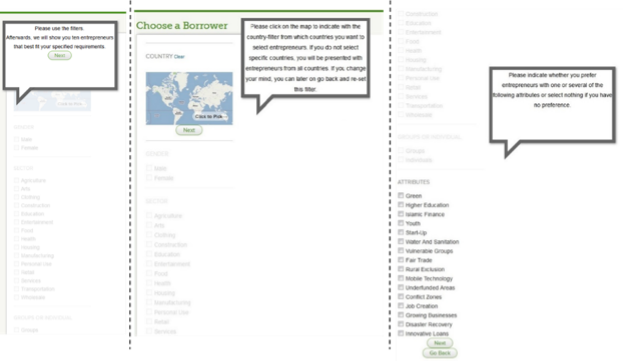
\includegraphics[width=0.8\textwidth]{graphics/Bild3.png}
    \caption{ Detailed Project Description Page with repayment schedule.}
    \label{fig:firststep}
\end{figure}

\begin{figure}[h]
    \centering
    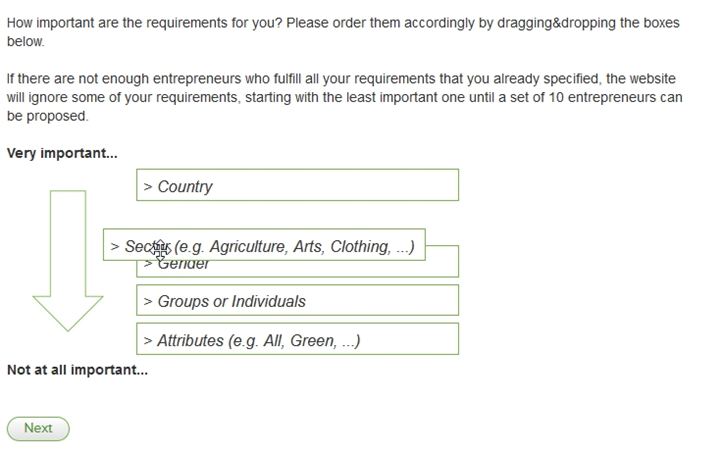
\includegraphics[width=0.8\textwidth]{graphics/Bild4.png}
    \caption{ Detailed Project Description Page with repayment schedule.}
    \label{fig:secondstep}
\end{figure}


\subsection{Procedure}
Figure \ref{fig:procedure2} illustrates the experimental
procedure. In addition to a lab session that lasted about 45 minutes, the
participants completed two short online surveys: a pre-questionnaire two weeks
before this session and a post questionnaire 12 weeks later. In the pre-questionnaire,
we asked participants what their goals would be when lending money, the
situation-specific thinking style they would use when deciding this, and other
control variables, like their age and gender. The two-week delay allowed us to
measure the constructs without making them overly salient during the lab study,
thereby reducing the risk that the elicitation of these constructs would
potentially influence participants during the lab session. In the post
questionnaire, we asked the participants how satisfied they still were with
their choice in the lab, and how often they had revisited the platform since
that time. We considered the 12-week delay between the lab session and the post
questionnaire sufficiently long to gauge the impact of our manipulations and of
any long-lasting effects resulting from the experience in the experiment. There
was no attrition between the pre-questionnaire and main experiment (the
pre-questionnaire was a pre-requisite in register for the experimental
session), but only 69 (78.4\%) of the 88 participants completed the post
questionnaire.\\
\begin{figure}[h]
    \centering
    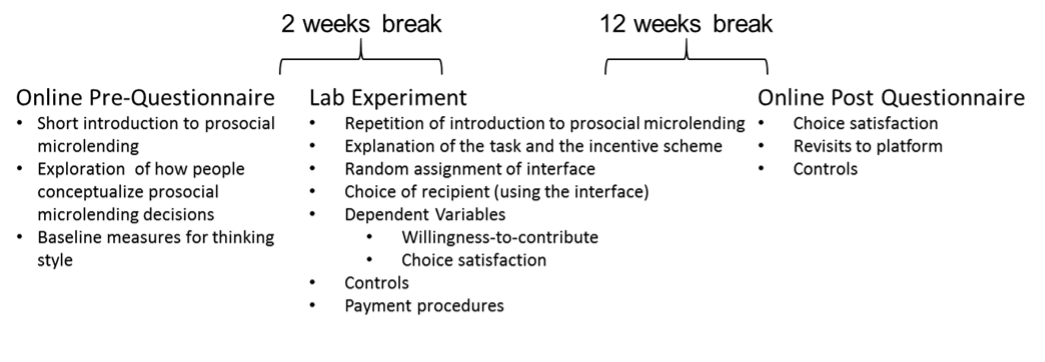
\includegraphics[width=0.8\textwidth]{graphics/Bild5}
    \caption{ Detailed Project Description Page with repayment schedule.}
    \label{fig:procedure2}
\end{figure}
\subsection{Results}
\bold{ Testing our Hypotheses}
Table \ref{tab:descriptive} shows
the descriptive statistics of the dependent variables and mediators that we use
for testing our hypotheses. In particular, we conceptualize analyticalStyle
(experientialStyle) as the change in analytical (experiential) thinking style
evoked by the interface in the main experiment. In particular, we calculate the
difference between the scores of the analytical (experiential) thinking style
scales of the pre-questionnaire and the main questionnaire. We see that, after
a choice has been made, the thinking style becomes less analytical (two-sided
t-test, $ t(87)=4.46, p<0.01 $ ) and slightly more experiential ($t(87)=-1.74,
p=0.09$). (A positive value indicates an increase in the analytical/experiential
thinking style after the participants had made their choice in the lab
experiment, compared to the one they had anticipated in the pre-questionnaire.)
Furthermore, Table \ref{tab:descriptive}
reveals that the perceived strategy restrictiveness is, with an average of
3.60, rather in the middle of the scale. In contrast, immediately after the
participants had made their choice, their choice satisfaction is relatively
high at 5.45, and also remains on a high level when asked again 12 weeks later
in the post questionnaire (both scales range from 1 to 7). Finally, the
participants were rather generous: On average, they contributed 60.81 to the
chosen project and only took 39.19 in cash.\\
\begin{table}[h]
    \centering
    \renewcommand{\arraystretch}{1.2} % Adjust row height for better readability

    \begin{tabular}{p{5cm} p{0.8cm} p{0.8cm} p{5cm} p{0.8cm} p{0.8cm}}
        \toprule
        \textbf{Variable} & \textbf{Mean} & \textbf{SD} & \textbf{Variable} & \textbf{Mean} & \textbf{SD} \\
        \midrule
        \multicolumn{6}{l}{\small{\textit{Dep var. variables and mediators (thinking style: [1,5], all others [1,7])}}} \\
        Analytical Style & -0.37 & 0.79 & Experiential Style & 0.12 & 0.65 \\
        Perceived Strategy Restrictiveness & 3.60 & 1.26 & Choice Satisfaction (Main Questionnaire) & 5.45 & 1.08 \\
        Choice Satisfaction (Post Questionnaire) & 5.00 & 1.27 & Willingness-to-Contribute & 60.81 & 25.11 \\
        \bottomrule
    \end{tabular}
        \caption{Descriptive statistics of mediators and dependent variables }
    \label{tab:descriptive}
\end{table}
To test our Hypotheses 1, 2, and 3 about the effects of the interfaces on the
different dimensions of the platform’s success, we conducted a separate OLS
regression for choice satisfaction and willingness-to-contribute. We computed
two models for choice satisfaction, one that regresses on the choice
satisfaction that was reported immediately after the choice in the lab (choice
satisfaction main) and one that regresses on the choice satisfaction reported
in the post questionnaire (choice satisfaction post). The STANDARD condition
was coded as the reference, so that the coefficients for NO-FILTER and SINGLE
reflect the respective differences when comparing these conditions with
STANDARD. In particular, the difference between the condition that supports an
attribute-based selection and the one that does not, is reflected in the
coefficient for NO-FILTER. The difference between the condition that supports
joint evaluation and the one that supports only single evaluation is reflected
in the coefficient for SINGLE. Table \ref{tab:hypothesis_results}
summarizes the results of the three models. … \\
\begin{table}[h]
    \centering
    \begin{tabular}{l c c c c c c}
        \hline
        & \multicolumn{2}{c}{Choice Sat. Main} & \multicolumn{2}{c}{Choice Sat. Post} & \multicolumn{2}{c}{WtC} \\
        Reference Category:\\ STANDARD & Coeff. & p-value & Coeff. & p-value & Coeff. & p-value \\
        \hline
        NO-FILTER & .039 & 0.887 & .131 & 0.727 & -3.42 & 0.603 \\
        SINGLE & -.618 & 0.029 & -.429 & 0.266 & 12 & 0.073 \\
        Constant & 5.60 & <0.010 & 5.10 & <0.010 & 57.92 & <0.010 \\
        N & 88 &  & 69 &  & 85 &  \\
        \hline
    \end{tabular}
    \caption{Results of Hypothesis 1, Hypothesis 2, and Hypothesis 3.}
    \label{tab:hypothesis_results}
\end{table}
\textbf{\textit{Additional Analyses}}

AND SO ON




